\documentclass[11pt,a4paper]{article}
\usepackage[margin=18mm,headheight=16pt]{geometry}
\usepackage{fontspec}
\setmainfont{DejaVu Sans}
\setsansfont{DejaVu Sans}
\setmonofont{DejaVu Sans Mono}[Scale=.80]
\usepackage[most]{tcolorbox}
\usepackage{xcolor,hyperref,fancyhdr,titlesec,enumitem,pdfpages,parskip}
\definecolor{navy}{HTML}{17365D}
\definecolor{teal}{HTML}{087E8B}
\definecolor{violet}{HTML}{7052A3}
\definecolor{orange}{HTML}{CC711F}
\definecolor{green}{HTML}{277D57}
\definecolor{paper}{HTML}{F4F8FC}
\hypersetup{colorlinks=true,linkcolor=navy,urlcolor=teal}
\pagestyle{fancy}\fancyhf{}\fancyhead[L]{\small\color{navy}MATH6342 | Linear Systems}\fancyhead[R]{\small Revision Guide}\fancyfoot[C]{\thepage}
\titleformat{\section}{\Large\bfseries\color{navy}}{\thesection}{1em}{}[\titlerule]
\titleformat{\subsection}{\large\bfseries\color{teal}}{\thesubsection}{.6em}{}
\tcbset{enhanced,breakable,boxrule=.65pt,arc=2.5mm,left=3mm,right=3mm,top=2mm,bottom=2mm,before skip=6pt,after skip=7pt}
\newtcolorbox{conceptbox}[1][]{colback=paper,colframe=teal,title={\bfseries Key explanation},#1}
\newtcolorbox{equationbox}[1][]{colback=violet!5,colframe=violet,title={\bfseries Formula / calculation},#1}
\newtcolorbox{exambox}[1][]{colback=orange!6,colframe=orange,title={\bfseries Exam method / worked solution},#1}
\newtcolorbox{proofbox}[1][]{colback=green!5,colframe=green,title={\bfseries Proof / reasoning},#1}
\newtcolorbox{studybox}[1][]{colback=navy!5,colframe=navy,title={\bfseries Revision checklist},#1}
\begin{document}
\begin{titlepage}\pagecolor{navy}\color{white}\vspace*{32mm}\begin{center}
{\Huge\bfseries MATH6342\\[4mm] Linear Systems}\\[14mm]
{\Large Visual Exam Revision Guide}\\[8mm]
{\large Simplified explanations, worked methods, proofs and exam checks}\\[22mm]
\begin{tcolorbox}[colback=white,colframe=white,width=.87\textwidth]\color{navy}\large Based on Gordon Blower's 2026/27 Lancaster University lecture slides. Includes a page-by-page companion and all 231 original lecture pages as appendices.\end{tcolorbox}
\vfill {\large LaTeX edition | October 2026}\end{center}\end{titlepage}\nopagecolor\color{black}
\tableofcontents\newpage
\begin{studybox}This is an expanded revision companion, not a guarantee of exam marks. Work through the original slides, proofs, assessed problems and past papers as well. The reference appendices preserve the detailed source material.\end{studybox}

\section{Complete, accessible revision companion}
\begin{conceptbox}Lancaster University · 2026/27 · Based on the 231-page lecture deck by Gordon Blower (5 October 2026).\end{conceptbox}
\begin{conceptbox}How this document is organised. The first part offers explanations, exam methods, fully worked examples, proof outlines, checks and questions. The second part preserves every page of the supplied lecture slides, in its original order, as a searchable reference appendix. The notes and slides should be studied together.\end{conceptbox}
\begin{conceptbox}Important: This is a teaching and revision supplement, not a prediction of examination questions. A high mark also requires practicing tutorial sheets, coursework and past papers, which were not included in the upload.\end{conceptbox}

\section{Course roadmap and study strategy}
\begin{studybox}• Chapter 1 (original slide frames 6–30): signals, feedback, differential equations, state-space and companion matrices.\end{studybox}
\begin{studybox}• Chapter 2 (frames 31–85): determinants, eigenvalues, norms, matrix exponentials, state-space solutions, transfer functions and realisation.\end{studybox}
\begin{studybox}• Chapter 3 (frames 86–134): Laplace transform definitions, algebraic rules, differential equations, convolution and inverse transforms.\end{studybox}
\begin{studybox}• Chapter 4 (frames 135–161): transfer functions, frequency responses, Nyquist/Bode plots and stability.\end{studybox}
\begin{studybox}• Chapter 5 (frames 162–218): feedback loops, polynomial tools, controller synthesis and stability including Lyapunov equations.\end{studybox}
\begin{studybox}• Appendices (frames 219–227): MATLAB commands and terminology.\end{studybox}
\begin{conceptbox}Four-pass revision: (1) Define every term without looking; (2) reproduce key theorems with their assumptions; (3) solve representative problems from scratch; (4) check your answer against physical meaning, units, dimensions and stability criteria. Rework every mistake after 48 hours.\end{conceptbox}

\section{Chapter 1 — Describing linear systems}

\subsection{1. Inputs, states, outputs and dimensions}
\begin{conceptbox}Think of a linear system as a machine with an external signal u(t), internal memory x(t), and observed response y(t). The state collects enough information to determine future behaviour if the future input is known.\end{conceptbox}
\begin{equationbox}\raggedright
{\ttfamily\small x'(t) = A x(t) + B u(t) y(t) = C x(t) + D u(t)}\par
\end{equationbox}
\begin{conceptbox}For n states, m inputs and p outputs: x is n×1, u is m×1, y is p×1; A is n×n, B is n×m, C is p×n, D is p×m. Always check dimensions before multiplying.\end{conceptbox}
\begin{conceptbox}A describes internal dynamics; B shows how input changes the state; C converts state to output; D is the direct input-to-output feedthrough.\end{conceptbox}

\subsection{2. What linearity really means}
\begin{equationbox}\raggedright
{\ttfamily\small L(a f + b g) = a L(f) + b L(g)}\par
\end{equationbox}
\begin{conceptbox}Both additivity and homogeneity are required. Differentiation, definite integration from 0 to t, multiplication by a fixed function, evaluation at a fixed instant, and fixed matrix multiplication are linear operators on suitable function spaces.\end{conceptbox}
\begin{conceptbox}A time-dependent coefficient does not automatically destroy linearity: y' = a(t)y + b(t)u is linear. A product y² or uy is nonlinear. An affine constant offset, such as y'=ay+1 without treating 1 as an input, does not describe a homogeneous linear map of state into derivative.\end{conceptbox}

\subsection{3. Block diagram language}
\begin{conceptbox}Amplifier = multiply signal by a coefficient. Integrator = accumulate signal over time. Differentiator = derivative. Summing junction = add signed branches. Tap = copy a signal without splitting its value. An arrow indicates the flow of information.\end{conceptbox}
\begin{conceptbox}An open-loop diagram contains no directed return path from downstream signals to earlier stages. A closed-loop system uses the output or state to modify what it receives. Positive feedback can increase response; negative feedback commonly opposes changes. Neither label alone proves stability.\end{conceptbox}
\begin{equationbox}\raggedright
{\ttfamily\small Positive feedback: y = u + θy => y = u/(1-θ) if θ ≠ 1.}\par
\end{equationbox}
\begin{equationbox}\raggedright
{\ttfamily\small Negative feedback: y = G(u-Hy) => y = [G/(1+GH)]u.}\par
\end{equationbox}
\begin{exambox}EXAM METHOD: label every internal arrow, write an equation at each summing junction and block, eliminate internal variables, and simplify. Never decide the denominator sign without writing the summing-junction equation.\end{exambox}

\subsection{4. From differential equations to state-space}
\begin{conceptbox}An nth-order scalar equation can be rewritten as n coupled first-order equations. The companion-matrix construction is the standard procedure.\end{conceptbox}
\begin{equationbox}\raggedright
{\ttfamily\small y\textasciicircum{}(n) + a\_(n-1)y\textasciicircum{}(n-1) + ... + a\_1 y' + a\_0 y = u}\par
\end{equationbox}
\begin{equationbox}\raggedright
{\ttfamily\small x = (y, y', ..., y\textasciicircum{}(n-1))\textasciicircum{}T; B=(0,...,0,1)\textasciicircum{}T}\par
\end{equationbox}
\begin{conceptbox}The companion matrix A has 1 on the superdiagonal, 0 in the remaining upper rows, and final row (-a\_0,-a\_1,...,-a\_(n-1)). The output for the original variable is y=(1,0,...,0)x.\end{conceptbox}
\begin{proofbox}The reason it works: the derivative of each state component is the next component, except the last derivative, which the original equation provides.\end{proofbox}

\subsection{Worked example: damped oscillator}
\begin{equationbox}\raggedright
{\ttfamily\small y'' + 3y' + 2y = u(t), x1=y, x2=y'}\par
\end{equationbox}
\begin{equationbox}\raggedright
{\ttfamily\small x1'=x2; x2'=-2x1-3x2+u}\par
\end{equationbox}
\begin{equationbox}\raggedright
{\ttfamily\small A=[[0,1],[-2,-3]], B=[[0],[1]], C=[1,0], D=0}\par
\end{equationbox}
\begin{conceptbox}The characteristic polynomial is λ²+3λ+2=(λ+1)(λ+2), so the unforced motion is a combination of exp(-t) and exp(-2t) and therefore decays. This is a quick physical sanity check.\end{conceptbox}

\subsection{Proof framework: reduction of order}
\begin{studybox}• State the differential equation and define x\_j=y\textasciicircum{}(j-1).\end{studybox}
\begin{studybox}• Differentiate x\_1,...,x\_(n-1) to get x\_j'=x\_(j+1).\end{studybox}
\begin{studybox}• Rearrange the original equation for x\_n', retaining the input term.\end{studybox}
\begin{studybox}• Write the resulting equations as x'=Ax+Bu and confirm sizes. This completes the derivation.\end{studybox}

\section{Chapter 2 — Solving systems with matrix theory}

\subsection{1. Determinants, cofactors, adjugates}
\begin{conceptbox}For a square matrix A, the determinant detects singularity: det A ≠ 0 exactly when A is invertible. Cofactor C\_ij equals (-1)\textasciicircum{}(i+j) times the determinant after removing row i and column j. The adjugate is the transpose of the cofactor matrix.\end{conceptbox}
\begin{equationbox}\raggedright
{\ttfamily\small A adj(A) = det(A) I; A\textasciicircum{}(-1)=adj(A)/det(A) when det A ≠ 0.}\par
\end{equationbox}
\begin{conceptbox}A triangular matrix has determinant equal to the product of its diagonal entries. Expand along a row or column with many zeros to minimise calculations.\end{conceptbox}

\subsection{2. Eigenvalues, characteristic polynomials and companion matrices}
\begin{equationbox}\raggedright
{\ttfamily\small χ\_A(λ) = det(λI-A) = λ\textasciicircum{}n - tr(A) λ\textasciicircum{}(n-1) + ... + (-1)\textasciicircum{}n det(A).}\par
\end{equationbox}
\begin{conceptbox}The course uses det(λI-A), not the alternate sign convention det(A-λI). Roots are eigenvalues. To get an eigenvector v for λ solve (A-λI)v=0; never divide by a singular matrix.\end{conceptbox}
\begin{conceptbox}Every monic polynomial λ\textasciicircum{}n+a\_(n-1)λ\textasciicircum{}(n-1)+...+a\_0 is the characteristic polynomial of its companion matrix. Hence one can turn a polynomial problem into a matrix problem.\end{conceptbox}

\subsection{3. Norms and stability bounds}
\begin{conceptbox}A vector norm measures the size of a vector. A compatible matrix operator norm measures its largest possible amplification of a vector: ||A||=sup\_\{||x||=1\}||Ax||. Key inequalities include ||Ax||≤||A||||x|| and ||AB||≤||A||||B||.\end{conceptbox}
\begin{conceptbox}Induced 1-norm is the maximum absolute column sum; induced infinity-norm is maximum absolute row sum; Euclidean operator norm is the largest singular value. For complex vectors, use conjugate transpose in inner products.\end{conceptbox}
\begin{conceptbox}A norm estimate can bound growth even if it does not determine the exact solution. Distinguish a bound from an equality.\end{conceptbox}

\subsection{4. Matrix exponentials and initial value problems}
\begin{equationbox}\raggedright
{\ttfamily\small exp(At) = I + At + (At)\textasciicircum{}2/2! + (At)\textasciicircum{}3/3! + ...}\par
\end{equationbox}
\begin{equationbox}\raggedright
{\ttfamily\small x(t)=exp(At)x(0) + ∫\_0\textasciicircum{}t exp(A(t-s)) B u(s) ds.}\par
\end{equationbox}
\begin{conceptbox}The first term is the free/homogeneous response determined by initial state; the integral is the forced response. If A=PΛP\textasciicircum{}(-1), then exp(At)=P diag(exp(λ\_i t)) P\textasciicircum{}(-1). If A has a Jordan block, polynomial factors in t can accompany exponentials.\end{conceptbox}
\begin{conceptbox}Check a proposed solution by differentiating and substituting into x'=Ax+Bu and verifying x(0). For constant A, d(exp(At))/dt=A exp(At).\end{conceptbox}

\subsection{Worked example: solve a diagonal system}
\begin{equationbox}\raggedright
{\ttfamily\small A=diag(-1,-2), B=(1,1)\textasciicircum{}T, u(t)=1, x(0)=(0,0)\textasciicircum{}T.}\par
\end{equationbox}
\begin{equationbox}\raggedright
{\ttfamily\small x1'=-x1+1 -> x1(t)=1-exp(-t).}\par
\end{equationbox}
\begin{equationbox}\raggedright
{\ttfamily\small x2'=-2x2+1 -> x2(t)=[1-exp(-2t)]/2.}\par
\end{equationbox}
\begin{conceptbox}At t=0 both components are zero; as t→∞ they tend to 1 and 1/2. The steady state is -A\textasciicircum{}(-1)B=(1,1/2)\textasciicircum{}T.\end{conceptbox}

\subsection{5. Outputs and transfer matrices}
\begin{equationbox}\raggedright
{\ttfamily\small x'=Ax+Bu, y=Cx+Du, zero initial state.}\par
\end{equationbox}
\begin{equationbox}\raggedright
{\ttfamily\small G(s)=C(sI-A)\textasciicircum{}(-1)B+D.}\par
\end{equationbox}
\begin{conceptbox}G is p×m. For a single input/single output (SISO), it is a rational function. For multiple inputs/outputs (MIMO), every entry is a rational function. Transfer functions describe the zero-initial-condition input/output behaviour; they do not, by themselves, disclose all hidden internal modes.\end{conceptbox}
\begin{conceptbox}A realization means finding A,B,C,D that generate a given G(s). Different state-space systems can produce the same transfer function. Check dimensions and calculate C(sI-A)\textasciicircum{}(-1)B+D explicitly.\end{conceptbox}

\subsection{Worked example: transfer function of an oscillator}
\begin{equationbox}\raggedright
{\ttfamily\small A=[[0,1],[-2,-3]], B=[[0],[1]], C=[1,0], D=0.}\par
\end{equationbox}
\begin{equationbox}\raggedright
{\ttfamily\small sI-A=[[s,-1],[2,s+3]], determinant = s²+3s+2.}\par
\end{equationbox}
\begin{equationbox}\raggedright
{\ttfamily\small (sI-A)\textasciicircum{}(-1)B = [1,s]\textasciicircum{}T/(s²+3s+2).}\par
\end{equationbox}
\begin{equationbox}\raggedright
{\ttfamily\small G(s)=1/(s²+3s+2)=1/[(s+1)(s+2)].}\par
\end{equationbox}
\begin{conceptbox}Always test the result against the ODE: taking the Laplace transform of y''+3y'+2y=u under zero initial conditions yields the same G(s).\end{conceptbox}

\section{Chapter 3 — Laplace transforms}

\subsection{1. Definition and existence}
\begin{equationbox}\raggedright
{\ttfamily\small L\{f\}(s)=F(s)=∫\_0\textasciicircum{}∞ exp(-st) f(t) dt.}\par
\end{equationbox}
\begin{conceptbox}Think of the transform as a way to replace differentiation by multiplication by s, while retaining initial values as correction terms. The variable s is usually complex; convergence requires sufficient decay of exp(-st)f(t).\end{conceptbox}
\begin{conceptbox}Typical transform pairs (for suitable Re(s)): L\{1\}=1/s; L\{exp(at)\}=1/(s-a); L\{t\textasciicircum{}n\}=n!/s\textasciicircum{}(n+1); L\{sin(ωt)\}=ω/(s²+ω²); L\{cos(ωt)\}=s/(s²+ω²).\end{conceptbox}

\subsection{2. Essential operational rules}
\begin{equationbox}\raggedright
{\ttfamily\small L\{af+bg\}=aF+bG.}\par
\end{equationbox}
\begin{equationbox}\raggedright
{\ttfamily\small L\{f'\}=sF-f(0); L\{f''\}=s²F-sf(0)-f'(0).}\par
\end{equationbox}
\begin{equationbox}\raggedright
{\ttfamily\small L\{exp(at) f(t)\}(s)=F(s-a).}\par
\end{equationbox}
\begin{equationbox}\raggedright
{\ttfamily\small L\{t f(t)\}(s) = -F'(s).}\par
\end{equationbox}
\begin{equationbox}\raggedright
{\ttfamily\small L\{∫\_0\textasciicircum{}t f(r)dr\}=F(s)/s.}\par
\end{equationbox}
\begin{conceptbox}Convolution is (f*g)(t)=∫\_0\textasciicircum{}t f(t-r)g(r)dr. Under appropriate conditions L\{f*g\}=F(s)G(s). This explains why cascaded linear time-invariant systems multiply their transfer functions.\end{conceptbox}

\subsection{Worked example: nonzero initial conditions}
\begin{equationbox}\raggedright
{\ttfamily\small y''+3y'+2y=1, y(0)=1, y'(0)=0.}\par
\end{equationbox}
\begin{equationbox}\raggedright
{\ttfamily\small (s²Y-s)+(3sY-3)+2Y=1/s.}\par
\end{equationbox}
\begin{equationbox}\raggedright
{\ttfamily\small Y(s)=[1/s+s+3]/[(s+1)(s+2)].}\par
\end{equationbox}
\begin{conceptbox}For the easiest time-domain solution, find the constant particular solution y\_p=1/2. The homogeneous solution is c1 exp(-t)+c2 exp(-2t). Using y(0)=1 and y'(0)=0 gives c1=1, c2=-1/2.\end{conceptbox}
\begin{equationbox}\raggedright
{\ttfamily\small y(t)=1/2 + exp(-t) - (1/2)exp(-2t).}\par
\end{equationbox}
\begin{conceptbox}Verify at t=0 and check the differential equation. In exams, forgetting the initial-value terms is a common major error.\end{conceptbox}

\subsection{3. Partial fractions and inverse transforms}
\begin{conceptbox}Factor the denominator. For a simple real pole at -a, A/(s+a) becomes A exp(-at). Repeated poles require A/(s+a)+B/(s+a)\textasciicircum{}2+...; the power k corresponds to t\textasciicircum{}(k-1)exp(-at)/(k-1)!.\end{conceptbox}
\begin{equationbox}\raggedright
{\ttfamily\small 1/[(s+1)(s+2)]=1/(s+1)-1/(s+2).}\par
\end{equationbox}
\begin{equationbox}\raggedright
{\ttfamily\small L\textasciicircum{}(-1)\{1/[(s+1)(s+2)]\}=exp(-t)-exp(-2t).}\par
\end{equationbox}
\begin{conceptbox}For irreducible quadratic factors, complete the square and compare with sine/cosine formulas. For improper rational functions, first use polynomial division before partial fractions.\end{conceptbox}

\subsection{4. Laplace transform of state-space models}
\begin{equationbox}\raggedright
{\ttfamily\small sX(s)-x(0)=AX(s)+BU(s).}\par
\end{equationbox}
\begin{equationbox}\raggedright
{\ttfamily\small X(s)=(sI-A)\textasciicircum{}(-1)x(0)+(sI-A)\textasciicircum{}(-1)BU(s).}\par
\end{equationbox}
\begin{equationbox}\raggedright
{\ttfamily\small Y(s)=C(sI-A)\textasciicircum{}(-1)x(0)+G(s)U(s).}\par
\end{equationbox}
\begin{conceptbox}The resolvent (sI-A)\textasciicircum{}(-1) connects the time-domain exponential and Laplace-domain algebra. Always separate the initial-state response from the input response.\end{conceptbox}

\section{Chapter 4 — Transfer functions and stability}

\subsection{1. Poles, zeros and minimal interpretation}
\begin{conceptbox}The poles of a reduced scalar rational transfer function are roots of its denominator; its zeros are roots of the numerator. A transfer function may show cancellations: they can conceal internal state dynamics, so distinguish input/output stability from internal stability.\end{conceptbox}
\begin{conceptbox}For a continuous-time finite-dimensional autonomous system x'=Ax, asymptotic stability holds when every eigenvalue of A has strictly negative real part. Eigenvalues with positive real part lead to growth. Imaginary-axis eigenvalues require more care; Jordan structure matters.\end{conceptbox}

\subsection{2. Frequency response}
\begin{equationbox}\raggedright
{\ttfamily\small If u(t)=exp(iωt), the steady-state output is related to G(iω).}\par
\end{equationbox}
\begin{conceptbox}Magnitude |G(iω)| describes gain, while arg G(iω) describes phase shift. For real sine-wave inputs one takes the appropriate real/imaginary part. The Fourier/frequency-response viewpoint helps interpret how a system treats slow and fast oscillations.\end{conceptbox}
\begin{conceptbox}Bode magnitude plots typically use 20 log10|G(iω)| in dB against logarithmic frequency; Bode phase plots show arg G(iω). A Nyquist plot traces G(iω) in the complex plane as frequency varies. The full Nyquist stability criterion needs its hypotheses and contour treatment; do not simply count crossings without defining the curve\end{conceptbox}
\begin{conceptbox}and open-loop poles.\end{conceptbox}

\subsection{Worked example: frequency response of a first-order filter}
\begin{equationbox}\raggedright
{\ttfamily\small G(s)=1/(s+2). G(iω)=1/(2+iω)=(2-iω)/(4+ω²).}\par
\end{equationbox}
\begin{equationbox}\raggedright
{\ttfamily\small |G(iω)|=1/sqrt(4+ω²), phase=-arctan(ω/2).}\par
\end{equationbox}
\begin{conceptbox}At ω=0, gain is 1/2; at large ω, gain tends to zero. The system suppresses high-frequency components. Its pole -2 lies in the left half-plane, so this first-order realization is asymptotically stable.\end{conceptbox}

\subsection{3. Stability workflow for exam questions}
\begin{studybox}• Identify the question: internal stability of A, BIBO stability of a transfer function, or stability of a closed feedback loop.\end{studybox}
\begin{studybox}• For internal stability compute the eigenvalues of the state matrix. For rational BIBO input/output stability inspect the poles after cancellation, subject to the stated assumptions.\end{studybox}
\begin{studybox}• For feedback derive the correct closed-loop denominator, often 1+G(s)H(s) for negative feedback.\end{studybox}
\begin{studybox}• Check the roots of the relevant characteristic polynomial. If using a frequency plot, state and apply the appropriate Nyquist assumptions.\end{studybox}
\begin{studybox}• Mention hidden unstable cancellations if the realisation is not known to be minimal.\end{studybox}

\section{Chapter 5 — Feedback control}

\subsection{1. Algebra of closed-loop systems}
\begin{equationbox}\raggedright
{\ttfamily\small e=r-Hy, u=K e, y=P u.}\par
\end{equationbox}
\begin{equationbox}\raggedright
{\ttfamily\small y=P K(r-Hy) -> (1+PKH)y=PKr.}\par
\end{equationbox}
\begin{equationbox}\raggedright
{\ttfamily\small T(s)=y/r=PK/(1+PKH).}\par
\end{equationbox}
\begin{conceptbox}Here P is the plant, K is the controller, H is the feedback/sensor element, and r is the reference. This algebra is valid for a scalar loop; in MIMO systems multiplication order matters and inverses are matrices.\end{conceptbox}

\subsection{Worked example: choose a proportional controller}
\begin{equationbox}\raggedright
{\ttfamily\small Plant P(s)=1/(s+2), unity negative feedback H(s)=1, K(s)=k.}\par
\end{equationbox}
\begin{equationbox}\raggedright
{\ttfamily\small T(s)=k/(s+2+k).}\par
\end{equationbox}
\begin{conceptbox}The closed-loop pole is -(2+k): for k>-2 it is strictly negative. Increasing positive k moves it left and speeds up the ideal first-order response, but the real-world trade-offs (noise, limits, uncertainty) are not captured by this elementary example.\end{conceptbox}
\begin{conceptbox}For a unit step, the steady-state output is k/(k+2) when stable, so proportional control alone leaves a steady-state tracking error of 2/(k+2).\end{conceptbox}

\subsection{2. Polynomial algebra and controller design}
\begin{conceptbox}The lecture sequence includes rational functions, greatest common divisors, Euclidean algorithms, matrix completion, and stabilising controller parameterisations. These techniques organise feedback design\end{conceptbox}
\begin{conceptbox}algebraically rather than relying exclusively on diagrams.\end{conceptbox}
\begin{conceptbox}To use the Euclidean algorithm on polynomials, divide P by Q to get P=SQ+R, where deg R<deg Q; replace (P,Q) by (Q,R) until remainder zero. The final nonzero remainder (normalised monic) is gcd(P,Q). Back-substitution yields Bézout coefficients X,Y with XP+YQ=gcd(P,Q).\end{conceptbox}
\begin{conceptbox}If gcd(P,Q)=1, a Bézout identity XP+YQ=1 proves coprimeness and can help solve stabilisation equations. In all controller problems, distinguish algebraic cancellation from physically acceptable/internal stability.\end{conceptbox}

\subsection{3. Lyapunov stability}
\begin{conceptbox}For x'=Ax, choose a real symmetric positive-definite matrix P and quadratic energy V(x)=x\textasciicircum{}T P x. Then V'=x\textasciicircum{}T(A\textasciicircum{}T P+PA)x.\end{conceptbox}
\begin{equationbox}\raggedright
{\ttfamily\small A\textasciicircum{}T P + P A = -Q, Q positive definite.}\par
\end{equationbox}
\begin{conceptbox}If P is also positive definite, then V>0 away from the origin and V'=-x\textasciicircum{}TQx<0 away from the origin, establishing asymptotic stability. For complex matrices use conjugate transpose A* and x*.\end{conceptbox}
\begin{conceptbox}For continuous-time Hurwitz A and a given Q>0, the Lyapunov equation has a unique positive-definite solution P. The lecture slides also discuss MATLAB calculations and related matrix equations.\end{conceptbox}

\subsection{Worked Lyapunov example}
\begin{equationbox}\raggedright
{\ttfamily\small A=diag(-1,-2), Q=I. Seek diagonal P=diag(p1,p2).}\par
\end{equationbox}
\begin{equationbox}\raggedright
{\ttfamily\small A\textasciicircum{}T P+PA=diag(-2p1,-4p2)=-I.}\par
\end{equationbox}
\begin{equationbox}\raggedright
{\ttfamily\small p1=1/2, p2=1/4; both positive.}\par
\end{equationbox}
\begin{equationbox}\raggedright
{\ttfamily\small V(x)=(1/2)x1²+(1/4)x2² and V'=-(x1²+x2²).}\par
\end{equationbox}
\begin{conceptbox}This proves asymptotic decay without explicitly solving the system.\end{conceptbox}

\subsection{4. MATLAB checks}
\begin{conceptbox}Common checks: eig(A) for eigenvalues; det(A) for determinant; expm(A*t) for matrix exponential; inv(s*eye(n)-A) when using symbolic variables; ss(A,B,C,D) and tf(...) when relevant toolboxes are available; bode, nyquist and step for system plots; lyap(A,Q) for the continuous Lyapunov equation A P+P A\textasciicircum{}T=-Q (note the exact transpose convention in each function).\end{conceptbox}
\begin{conceptbox}Use MATLAB to verify reasoning, not replace it: your written answer should state the mathematical criterion, show enough algebra, and interpret the result.\end{conceptbox}

\section{Proofs and concepts to practise from memory}
\begin{studybox}• Linearity of standard signal operators and reduction of a high-order ODE to first-order state-space.\end{studybox}
\begin{studybox}• Cofactor expansion and adjugate identity; characteristic polynomial of a companion matrix.\end{studybox}
\begin{studybox}• Existence and elementary properties of the matrix exponential; differentiation and solution of homogeneous systems.\end{studybox}
\begin{studybox}• Variation-of-constants formula for forced systems, with verification.\end{studybox}
\begin{studybox}• Laplace derivative rule via integration by parts and convolution multiplication rule.\end{studybox}
\begin{studybox}• Derivation of G(s)=C(sI-A)\textasciicircum{}(-1)B+D from zero initial conditions.\end{studybox}
\begin{studybox}• Closed-loop transfer algebra with feedback sign explicitly indicated.\end{studybox}
\begin{studybox}• Quadratic Lyapunov proof using positive-definite P and Q.\end{studybox}
\begin{studybox}• Conditions needed before applying frequency-domain stability tests.\end{studybox}

\section{Self-test: 12 exam-style questions}

\subsection{1. Give dimensions of A,B,C,D when x∈R\textasciicircum{}4, u∈R\textasciicircum{}2, y∈R\textasciicircum{}3.}
\begin{exambox}Solution: A 4×4, B 4×2, C 3×4, D 3×2.\end{exambox}

\subsection{2. Is Lf(t)=t f(t) linear? Is Lf(t)=f(t)\textasciicircum{}2 linear?}
\begin{exambox}Solution: The first is linear for fixed t-multiplier; the square is nonlinear.\end{exambox}

\subsection{3. Convert y''+4y'+5y=u into companion state-space.}
\begin{exambox}Solution: x=(y,y')\textasciicircum{}T; A=[[0,1],[-5,-4]], B=(0,1)\textasciicircum{}T, C=(1,0), D=0.\end{exambox}

\subsection{4. Find eigenvalues of A=diag(-2,3). Is x'=Ax stable?}
\begin{exambox}Solution: -2 and 3. Unstable because one eigenvalue has positive real part.\end{exambox}

\subsection{5. Compute exp(At) for A=diag(-1,-3).}
\begin{exambox}Solution: diag(exp(-t),exp(-3t)).\end{exambox}

\subsection{6. Find G(s) for y'+5y=2u and y(0)=0.}
\begin{exambox}Solution: G(s)=2/(s+5).\end{exambox}

\subsection{7. Find L\{t exp(-2t)\}.}
\begin{exambox}Solution: 1/(s+2)\textasciicircum{}2.\end{exambox}

\subsection{8. Find inverse Laplace of 1/[(s+2)(s+3)].}
\begin{exambox}Solution: exp(-2t)-exp(-3t).\end{exambox}

\subsection{9. Derive closed-loop negative-feedback transfer for P and H.}
\begin{exambox}Solution: P/(1+PH), with the controller incorporated into P if appropriate.\end{exambox}

\subsection{10. Find closed-loop pole for P(s)=1/(s+4), unity feedback K=k.}
\begin{exambox}Solution: Pole = -(4+k), stable for k>-4.\end{exambox}

\subsection{11. Find the magnitude of G(iω) if G(s)=3/(s+1).}
\begin{exambox}Solution: 3/sqrt(1+ω²).\end{exambox}

\subsection{12. Solve A\textasciicircum{}TP+PA=-I with A=-2 (scalar).}
\begin{exambox}Solution: P=1/4>0; V=x²/4 decreases as x'=-2x.\end{exambox}

\section{Common marking pitfalls}
\begin{studybox}• Not stating zero-initial-state assumption when deriving a transfer function.\end{studybox}
\begin{studybox}• Writing χ\_A as det(A-λI) without noting the sign convention.\end{studybox}
\begin{studybox}• Using incorrect companion-matrix coefficient order or signs.\end{studybox}
\begin{studybox}• Ignoring input/output/matrix dimensions, especially in MIMO products.\end{studybox}
\begin{studybox}• Confusing eigenvalues of A with poles of a reduced, possibly nonminimal transfer function.\end{studybox}
\begin{studybox}• Dropping y(0) and y'(0) in Laplace transformations.\end{studybox}
\begin{studybox}• Treating positive/negative feedback as automatically stable/unstable.\end{studybox}
\begin{studybox}• Using a Lyapunov equation without verifying positive definiteness.\end{studybox}
\begin{studybox}• Reporting numerical software outputs without explaining the mathematical principle.\end{studybox}

\section{How to use the complete original-slide appendix}
\begin{conceptbox}Every original slide follows after this revision section, in the exact sequence supplied. Work through frames 1–227 (including repeated numbering), paying special attention to propositions and proofs, the detailed MATLAB appendix and the glossary. Use the appendix to examine diagrams, examples, exact hypotheses, and any material that is only summarised here.\end{conceptbox}
\begin{conceptbox}This companion prioritises conceptual explanation and representative exam methods. The appended slides provide comprehensive source coverage; studying only the companion summaries would not be a substitute for mastering every technical theorem in Chapter 5.\end{conceptbox}

\clearpage\section*{Slide-by-slide lecture walkthrough}\addcontentsline{toc}{section}{Slide-by-slide lecture walkthrough}
The following reference section preserves the 36-page slide-by-slide reading companion from the earlier revision document. It is included as a PDF appendix (rather than editable text).
\includepdf[pages=-,pagecommand={},scale=.94]{_linear_slide_walkthrough.pdf}
\clearpage\section*{Original MATH6342 Lecture Slides}\addcontentsline{toc}{section}{Original MATH6342 Lecture Slides}
All 231 pages of the supplied university lecture slide deck follow, unchanged. These pages are embedded PDF source material, not editable LaTeX content.
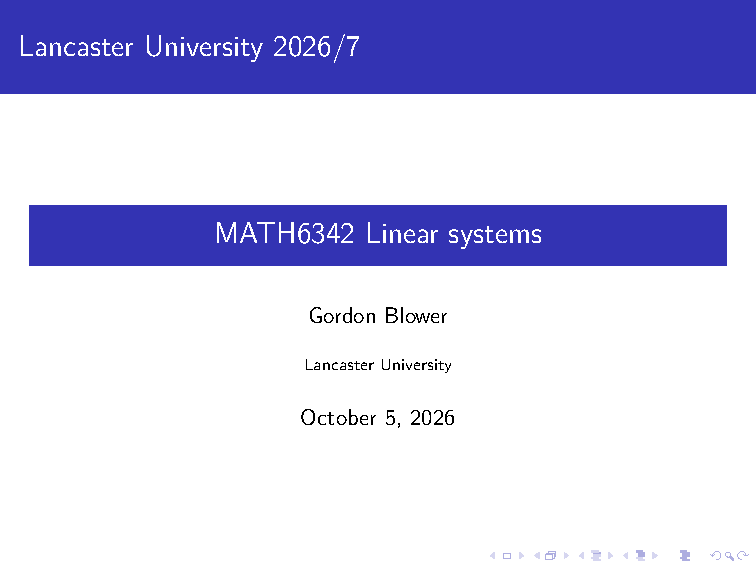
\includepdf[pages=-,pagecommand={},fitpaper=true]{MATH6342 Linear systems beamer (3).pdf}
\end{document}
